\section{线性谐振子}

\subsection{胡克定律}

中学里我们都学过胡克定律(Hooke's Law),一个弹簧,下面挂个重物,假设弹簧原来的长度是$x_0$,弹簧被拉抻的长度$\Delta x = x - x_0$和重物的重量成正比。表示成数学式子就是:

\begin{equation}
F = - k \Delta x
\end{equation}

这里$F$是弹簧的弹性力,它的方向和弹簧拉抻的方向相反,所以要有个负号“$-$”,$k$是弹性系数,表示弹簧的“软硬”,弹簧越“硬”,$k$就越大,所谓“强弓硬弩”,弹簧越硬,我们只需稍稍使弹簧有个拉抻,它就会有个很大的弹力。$\Delta x$就是拉抻,如果是在重力场中,弹簧会向下被拉长。

弹簧是人类使用的最早的储能器,比如在希腊-罗马时期,西方就懂得制作大型的弩炮,并懂得利用绷紧皮筋发出的声音校准弩炮射击的方向。维特鲁威是罗马时期的建筑师,同时他也是给罗马军团制造大型弩炮的工匠,在他的《建筑十书》中曾有这样的记录:

\begin{quote}
将皮筋绳索穿入(弹索孔),并以绞车和杠杆将其绷紧,绷到弩炮制作者能听到皮筋绳索发出特定音高的弦音,方可用楔子将它固定住。将弩炮的双臂扣上扳机,一旦发射,两边皮筋就应释放出一致的推力。如果它们发出的音调不一致,弩炮射出的弹丸便不可能是直线的。
\end{quote}

\begin{figure}[htbp]
\begin{center}
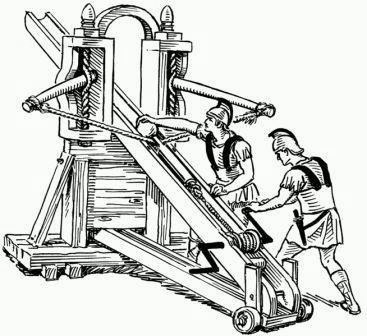
\includegraphics[width=10cm]{LinearOscillator/roman-catapult.png}
\caption{罗马军团的小型弩炮}
%\label{default}
\end{center}
\end{figure}

我们可以把弩炮的皮筋看做是左右两段,只有当左右两段上的张力大小相等时,弩炮才好瞄准。维特鲁威这里叙述的方法是通过分辨张紧弦音的高低来判断左右两段弦是否具有大小相等的张力的。如果音高相同,即说明左右两段弦上的张力相同。

让我们重新回到弹簧,重新选择位置的原点是$x_0 = 0$,形变$\Delta x = x$弹簧中储存的能量是:

\begin{equation}
- \int_0^x F(x')d x' = \int_0^x k x' d x' = \frac{k x^2}{2} 
\end{equation}

这个能量和位置有关,我们称之为势能,记作$V(x)$。假设弹簧本身的重量忽略不计,弹簧上悬挂的重物质量为$m$,质量为$m$的物体运动起来,会有动能$T$:

\begin{equation}
\frac{m {\dot x}^2}{2}
\end{equation}

这里$\dot x$表示对位置的求导,即速度。考虑到动量$p = m \dot x$,动能项可以写成:

\begin{equation}
\frac{p^2}{2m}
\end{equation}

根据经典力学中的哈密顿形式,哈密顿量可写为:动能项+势能项:

\begin{equation}
H = \frac{p^2}{2m} + \frac{kx^2}{2}
\end{equation}

这个表达式可以看做是对线性谐振子的定义,很多实际问题可以近似地看做是个线性谐振子的问题(比如单摆和弹簧),或好多线性谐振子的相互耦合(比如绷紧的弦和弹簧床)。

我们先来求“线性谐振子”的经典解,根据哈密顿力学:

\begin{eqnarray}
\dot x &=& \frac{\partial H}{\partial p} = \frac{p}{m}\\
\dot p &=& - \frac{\partial H}{\partial x} = - kx
\end{eqnarray}

由上式,我们可得到:

\begin{equation*}
\dot p = m \ddot x = - k x
\end{equation*}

即:

\begin{equation}
\ddot x + \omega^2 x = 0
\end{equation}

这是一个标准的二阶微分方程,可以解出:

\begin{equation}
x = A \cos \omega t + B \sin \omega t
\end{equation}

这里A和B都是待定常数,由线性谐振子的初始运动状况(初始位置和初始动量)决定。

$\omega$是简谐振动的振动频率:

\begin{equation}
\omega = \sqrt{\frac{k}{m}}
\end{equation}

在此基础上我们把线性谐振子的哈密顿量写为:

\begin{equation}
H = \frac{p^2}{2m} + \frac{m \omega^2 x^2}{2}
\end{equation}

现在我们就知道所谓“线性谐振子”指的是:

\begin{enumerate}

\item 

弹性回复力和位移成正比,就是线性。

\item

求解出来的运动是周期性的简谐振动,就是谐振子。

\end{enumerate}

下面我们就要研究线性谐振子的量子力学求解了,但在此之前我们先回顾下(或重新讨论下)基础对易式和薛定谔方程。

\subsection{基础对易式和不确定关系}

\subsubsection{平移算符}

在量子力学中,一个物理系统的运动状态是由态矢量$\left| \alpha \right\rangle$刻画的,它可以处在空间的某个位置上,并随时间演化。

我们先来研究态矢量在空间位置上的平移,假想我们自己就是态矢量,我们可以往前走走,或等效地我们可以想象让坐标框架往后动动。

定义平移算符$T$,$T(\delta)$使态矢量向前移动了无穷小距离$\delta$,使得:

\begin{equation}
\left| \alpha, \delta \right\rangle = T(\delta) \left| \alpha \right\rangle 
\end{equation}

假设在空间中移动态矢量并不会导致态矢量本身大小的改变,原来是归一的态矢量,现在还是归一的态矢量。

\begin{equation}
\left\langle \alpha | \alpha \right\rangle = \left\langle \alpha, \delta | \alpha, \delta \right\rangle = \left\langle \alpha \right| T^\dagger(\delta) T(\delta) \left| \alpha \right\rangle    
\end{equation}

这个条件要求平移算符是幺正的(Unitary)。

\begin{equation}
T^\dagger (\delta) T (\delta ) =  1
\end{equation}

考虑到位置是个连续变量\footnote{对态矢量的平移操作不会改变态矢量的归一性,及平移可以取无限小都是对我们所处的物理空间的性质的假设。这些假设也是康德先验空间概念的具体化。},我们可以要求$\delta \to 0$,然后把$\delta$看做是小量展开,并略去所有的高阶小量(在这里就是$\delta^2$及$\delta$的更高幂次的项)。

假设$T(\delta)$可表示为:

\begin{eqnarray}
T(\delta) & = & 1- i K \delta \\
T^\dagger (\delta) & = & 1+ i K^\dagger \delta
\end{eqnarray}

代入$T^\dagger T =1$的表达式中:

\begin{equation*}
\left( 1+ i K^\dagger \delta \right) \left( 1- i K \delta \right) = 1 + i \left( K^\dagger - K \right) \delta = 1
\end{equation*}

这意味着:

\begin{equation}
K^\dagger = K
\end{equation}

即$K$是个厄米算符,可以对应一个物理量的取值。从量纲的角度考虑,$K$所对应物理量的量纲应该是[长度]$^{-1}$,即波矢$k = \frac{2 \pi}{ \lambda }$的量纲。考虑到$p = \hbar k$,我们可以把厄米算符$K$定义为:

\begin{equation}
K = \frac{P}{\hbar}
\end{equation}

这里$P$是动量算符。

\subsubsection{基础对易式}

考虑位置算符$X$,它使得:

\begin{equation}
X \left| x' \right\rangle = x' \left| x' \right\rangle 
\end{equation}

这其实就是位置算符的本征值问题,求出来本征值是$x'$,本征矢$\left| x' \right\rangle$。

在此基础上考虑如下运算:

\begin{eqnarray*}
X T(\delta) \left| x' \right\rangle &=& X \left| x' + \delta \right\rangle = \left( x' + \delta \right) \left| x' + \delta \right\rangle \\
T(\delta) X \left| x' \right\rangle &=& x' T(\delta) \left| x' \right\rangle = x' \left| x' + \delta \right\rangle  
\end{eqnarray*}

把上面两个表达式相减就是:

\begin{equation*}
\left( XT - TX \right) \left| x' \right\rangle = \delta \left| x' + \delta \right\rangle  
\end{equation*}

上式的右侧有两个$\delta$,我们需要把它展开到$\delta$的一次,并忽略$\delta^2$及以上的项。

\begin{equation*}
\delta \left| x' + \delta \right\rangle = \delta \left( 1- i K \delta \right) \left| x' \right\rangle = \delta \left| x' \right\rangle
\end{equation*}

现在等式两边都展开到$\delta$的一次:

\begin{equation*}
XT - TX = X \left( 1- i K \delta \right) - \left( 1- i K \delta \right) X = -i XK \delta + i KX \delta
\end{equation*}

完整写出来:

\begin{equation*}
\left( -i XK + i KX \right) \delta \left| x' \right\rangle = \delta \left| x' \right\rangle
\end{equation*}

这意味着:

\begin{equation}
XK - KX = i
\end{equation}

改写成动量的形式($\hbar K \to P$):

\begin{equation}
XP - PX = i \hbar
\end{equation}

这就是量子力学中的基础对易式(the fundamental commutator),我们一般把它写为:

\begin{equation}
\left[ X, P \right] = i \hbar
\end{equation}

\subsubsection{不确定关系}

由基础对易式出发,我们可以严格地推导海森堡不确定关系(uncertainty relation)。

不确定关系讲的是,假如我们测量粒子的位置的话,如果我们确定地(几率为1地)知道粒子在哪儿的话,那么我们就完全不知道粒子的动量了。

相反如果我们确定地知道粒子的动量是多少的话,我们就完全不知道粒子的位置了。因此有个笑话,讲警察抓住物理学家超速。这个物理学家会跟警察这么argue:

\begin{enumerate}
\item 

你确定我的车是在这里吗?如果你确定,那你就不知道我的车有多快。

\item

你确定我的车速是这么快吗?如果你确定,那你就不能说我的车在限速区里。

\end{enumerate}

换句话说我们只能在一定限度内知道粒子的位置和粒子的动量,粒子位置的不确定度和粒子动量的不确定度相乘满足如下不等式:

\begin{quotation}
位置的不确定度 $\times$ 动量的不确定度 $\ge $ h
\end{quotation}

首先这不是一个精确的关系,其次我们需要定义什么是位置的不确定度。

对任意态矢量$\left| \alpha \right\rangle$我们能计算位置$X$的量子力学平均$\left\langle X \right\rangle$:

\begin{equation}
\left\langle X \right\rangle = \left\langle \alpha \right| X \left| \alpha \right\rangle
\end{equation}

那么位置对平均位置的偏离$\Delta X$可以用来刻画位置的不确定度吗?

\begin{equation}
\Delta X = X  -  \left\langle X \right\rangle
\end{equation}

$\Delta X$是厄米算符,其量子力学平均可正可负,平均来说是0,

\begin{equation*}
\left\langle X -  \left\langle X \right\rangle \right\rangle = \left\langle X \right\rangle - \left\langle X \right\rangle = 0
\end{equation*}

我们没法用$\Delta X$来表征“位置的不确定度”,但我们可以考虑$\left( \Delta X  \right)^2 $,它是非负的。

\begin{equation}
\left\langle  \left( \Delta X  \right)^2  \right\rangle = \left\langle X^2 \right\rangle - \left\langle X \right\rangle^2
\end{equation}

类似地,我们也可以考虑$\left( \Delta P \right)^2 $,用$\sigma_X = \sqrt{ \left\langle  \left( \Delta X  \right)^2  \right\rangle  }$表示位置的不确定度,用$\sigma_P = \sqrt{ \left\langle  \left( \Delta P  \right)^2  \right\rangle  }$表示动量的不确定度。

定义:

\begin{eqnarray*}
\Delta X \left| \alpha \right\rangle &=& \left| \gamma \right\rangle \\
\Delta P \left| \alpha \right\rangle &=& \left| \delta \right\rangle
\end{eqnarray*}

对于态矢量$\left| \gamma \right\rangle$,$\left| \delta \right\rangle$存在不等式:

\begin{equation}
\left\langle \alpha | \alpha \right\rangle \left\langle \beta | \beta \right\rangle \ge \left| \left\langle \alpha | \beta \right\rangle \right|^2
\end{equation}

这个式子叫施瓦茨不等式(Schwarz inequality),有很直观的含义,比如在三维空间中:假设有$a$,$b$两个向量,它们之间的夹角是$\theta_{ab}$,由于$\cos \theta_{ab} \le 1$,我们有:

\begin{equation}
\left( a \cdot a \right) \left( b \cdot b \right) \ge \left| a \cdot b  \right|^2
\end{equation}

现在我们有:

\begin{equation*}
\left\langle \left( \Delta X \right)^2  \right\rangle \left\langle \left( \Delta P \right)^2  \right\rangle \ge \left|  \left\langle \Delta X \Delta P \right\rangle  \right|^2
\end{equation*}

除了对易式,

\begin{equation}
\left[ A, B \right] = AB - BA
\end{equation}

我们还可以定义反对易式:

\begin{equation}
\{ A, B \} = AB + BA
\end{equation}

我们现在有:

\begin{equation}
AB = \frac{\left[ A, B \right] + \{ A, B \} }{2}
\end{equation}

假设A,B都是厄米算符,我们可以证明$\{ A, B \}$也是厄米的:

\begin{equation*}
\left( \{ A, B \} \right)^\dagger = \left( AB + BA \right)^\dagger = BA + AB = \{ A, B \}
\end{equation*}

但$\left[ A, B \right]$是反厄米的:

\begin{equation*}
\left( \left[ A, B \right] \right)^\dagger = \left( AB - BA \right)^\dagger = BA - AB = -  \left[ A, B \right]
\end{equation*}

所谓反厄米算符的定义就是:

\begin{equation}
C^\dagger = -C
\end{equation}

给定态矢量$\left| \alpha \right\rangle$,对反厄米算符$C$计算“量子力学平均”:

\begin{equation*}
\left\langle \alpha | C \alpha \right\rangle = \left\langle \alpha C^\dagger |  \alpha \right\rangle = - \left\langle \alpha C |  \alpha \right\rangle = - \left\langle \alpha | C \alpha \right\rangle^* 
\end{equation*}

假设$\left\langle \alpha | C \alpha \right\rangle = a + i b$,$\left\langle \alpha | C \alpha \right\rangle^* = a - i b$,对反厄米算符$C$,满足:$\left\langle \alpha | C \alpha \right\rangle = a + ib = -a + ib$,实部$a$必须为0。

因此我们得到一个重要结论,对反厄米算符而言,其量子力学平均是个纯虚数。

这意味着$\left\langle \Delta X \Delta P \right\rangle$里有两项,一项是纯虚数,是反厄米算符$\frac{\left[ \Delta X, \Delta P \right]}{2}$的贡献,另一项是实数,是厄米算符$\frac{\{ \Delta X, \Delta P \}}{2}$的贡献。

现在关于$\left\langle \left( \Delta X \right)^2  \right\rangle \left\langle \left( \Delta P \right)^2  \right\rangle$的不等式就变为:

\begin{equation*}
\left\langle \left( \Delta X \right)^2  \right\rangle \left\langle \left( \Delta P \right)^2  \right\rangle \ge \left|  \left\langle \Delta X \Delta P \right\rangle  \right|^2 \ge \frac{1}{4} \left| { \left\langle { \left[ \Delta X, \Delta P \right] } \right\rangle } \right|^2
\end{equation*}

对于位置算符和动量算符而言,满足:

\begin{equation*}
\left[ \Delta X, \Delta P \right] = \left[ X, P \right] = i \hbar
\end{equation*}

因此:

\begin{equation}
\sigma_X \sigma_P = \sqrt{ \left\langle \left( \Delta X \right)^2 \right\rangle } \sqrt{ \left\langle \left( \Delta P \right)^2  \right\rangle }  \ge \frac{\hbar}{2}
\end{equation}

上式就是严格的海森堡不确定关系。

利用不确定关系,可以进行很多简单的估算,比如我们现在就来估算一下线性谐振子的基态能(ground state energy)。

首先谐振子的能量可近似地表示为:

\begin{equation}
E = \frac{\sigma_P^2 }{2m} + \frac{m \omega^2 \sigma_X^2}{2}
\end{equation}

利用关系:

\begin{equation}
a^2 + b^2 \ge 2 a b
\end{equation}

把线性谐振子的能量重新表示为:

\begin{equation}
E = \frac{\sigma_P^2 }{2m} + \frac{m \omega^2 \sigma_X^2}{2} \ge \omega \sigma_X \sigma_P \ge \frac{\hbar \omega}{2}
\end{equation}

这意味着线性谐振子的能量存在着一个非零的最小值,即基态能$\frac{\hbar \omega}{2}$。这个结果和经典线性谐振子的结果形成了鲜明的对照,在经典线性谐振子中,$x = 0$且$p=0$这样的态是可以存在的,但在量子力学中由于不确定原理的限制,我们不能让粒子的位置和动量同时取确定值,那么它就必须“振动”起来,我们管这种运动叫做“零点振动”。

\subsection{运动方程}

我们现在来考虑量子态随时间演化的问题。

假设时刻$t$,量子态是$\left| \alpha, t \right\rangle$,时刻$t + \epsilon$,量子态是$\left| \alpha, t+\epsilon \right\rangle$。定义演化算符$U(\epsilon)$,使得:

\begin{equation}
\left| \alpha, t + \epsilon \right\rangle = U(\epsilon ) \left| \alpha, t \right\rangle
\end{equation}

假设我们能够很好地追踪量子态随时间的演化,在演化的过程中没有“分叉”,也没用“汇聚”,即假设原先$\left| \alpha, t \right\rangle$是归一的话,演化$\epsilon$后,态$\left| \alpha, t + \epsilon \right\rangle$仍是归一的:

\begin{equation}
\left\langle \alpha, t | \alpha, t \right\rangle =  \left\langle \alpha, t + \epsilon | \alpha, t + \epsilon \right\rangle = \left\langle \alpha, t \right| U^\dagger (\epsilon ) U(\epsilon) \left| \alpha, t \right\rangle = 1 
\end{equation}

这就要求时间演化算符$U$是幺正的:

\begin{equation}
U^\dagger (\epsilon) U (\epsilon) = 1
\end{equation}

由于时间也是可以连续取值的,我们取$\epsilon \to 0$,并在以下运算中展开到$\epsilon$的一次方,忽略$\epsilon$的更高次的贡献。

假设$U(\epsilon) $可表示为:

\begin{eqnarray}
U(\epsilon) &=& 1 - i \Omega \epsilon \\
U^\dagger (\epsilon) &=& 1 + i \Omega^\dagger \epsilon
\end{eqnarray}

代入幺正条件$U^\dagger U =1$:

\begin{equation*}
\left( 1+ i \Omega^\dagger \epsilon \right) \left( 1 - i \Omega \epsilon  \right) = 1 + i \left( \Omega^\dagger - \Omega \right) \epsilon = 1
\end{equation*}

这意味着:

\begin{equation}
\Omega^\dagger = \Omega
\end{equation}

即算符$\Omega$是厄米算符,可以定义一个物理量与之对应。从量纲的角度,$\epsilon$的量纲是[时间],$\Omega$对应物理量的量纲就是[时间]$^{-1}$。考虑到$E = \hbar \omega$,我们可以把厄米算符$\Omega$定义为:

\begin{equation}
\Omega = \frac{H}{\hbar}
\end{equation}

这里$H$是哈密顿算符(哈密顿算符的本征值是能量)。

考虑:

\begin{equation*}
\left| \alpha, t + \epsilon \right\rangle = U(\epsilon ) \left| \alpha, t \right\rangle = \left( 1- i \Omega \epsilon \right) \left| \alpha, t \right\rangle
\end{equation*}

整理可得:

\begin{equation*}
\frac{ \left| \alpha, t + \epsilon \right\rangle - \left| \alpha, t \right\rangle }{\epsilon} = - i \frac{H }{\hbar} \left| \alpha, t \right\rangle
\end{equation*}

即:

\begin{equation}
i \hbar \frac{\partial }{\partial t} \left| \alpha, t \right\rangle = H \left| \alpha, t \right\rangle
\end{equation}

这是一个关于$t$的一阶偏微分方程,形式地解出:

\begin{equation}
\left| \alpha , t \right\rangle = e^{- \frac{i H t}{\hbar}} \left| \alpha \right\rangle = U(t ) \left| \alpha \right\rangle
\end{equation}

这里$U(t)$是有限时间的演化算符,由时刻$0$演化到时刻$t$:

\begin{equation}
U (t) = e^{- \frac{i H t}{\hbar}}
\end{equation}

\begin{figure}[htbp]
\begin{center}
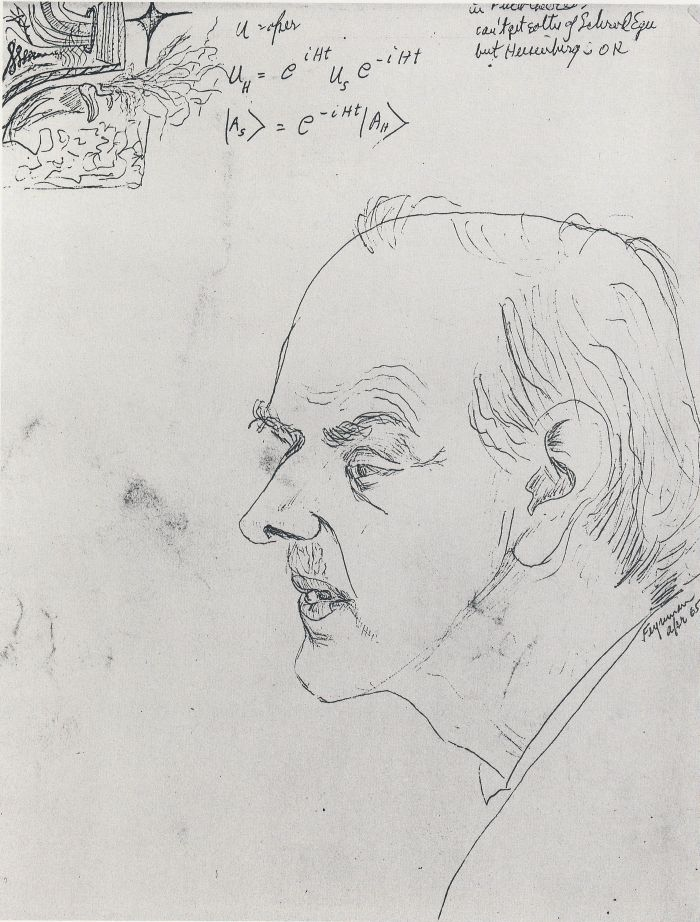
\includegraphics[width=10cm]{Spin/DbyF.jpg}
\caption{费曼画的狄拉克,图的左上角有演化算符。}
%\label{default}
\end{center}
\end{figure}

现在对量子态$\left| \alpha, t \right\rangle$计算某个物理量$A$的量子力学平均:

\begin{equation}
\left\langle A \right\rangle = \left\langle \alpha, t \right| A \left| \alpha, t \right\rangle = \left\langle \alpha \right| U^\dagger(t) A U(t) \left| \alpha \right\rangle
\end{equation}

这里的$A$就是位置算符$X$,动量算符$P$等,形式上它们与时间无关,现在我们定义一个形式上和时间有关的算符$A(t)$:

\begin{equation}
A(t) = U^\dagger (t ) A U(t)
\end{equation}

此时态矢量$\left| \alpha \right\rangle$在形式上就和时间无关了,它是$t=0$时候的$\left| \alpha, t \right\rangle$,

\begin{equation}
\left| \alpha \right\rangle = \left| \alpha, t = 0 \right\rangle
\end{equation}

此时物理系统随时间的演化将由算符$A(t)$随时间的演化描述。这种描述量子系统随时间演化的方式叫做海森堡绘景(Heisenberg picture)。与之相对的,算符$A$不随时间变化,但态矢量$\left| \alpha, t \right\rangle $随时间变化的描述方式叫做薛定谔绘景(Sch$\ddot o$dinger picture)。

现在我们来计算海森堡绘景下物理量$A(t)$是如何随时间演化的:

\begin{equation*}
\frac{\partial A(t) }{\partial t }  = \left( \frac{ \partial U^\dagger }{\partial t } \right) A U + U^\dagger A \left( \frac{ \partial U }{\partial t } \right)
\end{equation*}

对$U(t) = e^{- \frac{i H t}{\hbar}}$,我们可以计算:

\begin{eqnarray}
\frac{\partial U }{\partial t } &=& - \frac{i H U}{\hbar}  \\
\frac{\partial U^\dagger }{\partial t } &=& \frac{i U^\dagger H }{\hbar}
\end{eqnarray}

代入对$A(t)$微分:

\begin{equation*}
\frac{\partial A(t) }{\partial t } = \frac{i}{\hbar} \left( U^\dagger H AU - U^\dagger A H U \right)
\end{equation*}

考虑到$U^\dagger U = U U^\dagger  = 1$,

\begin{equation*}
i \hbar \frac{\partial A(t) }{\partial t }  = U^\dagger A U U^\dagger H U - U^\dagger H U U^\dagger A U = A(t)H(t) - H(t)A(t) 
\end{equation*}

为了书写的简单,我们往往就把$A(t)$写为$A$,这样就得到标准的物理量随时间演化的方程:

\begin{equation}
\dot A = \frac{\left[ A, H  \right]}{i \hbar} 
\end{equation}

这个方程就是著名的海森堡运动方程(Heisenberg equation of motion)。

\subsection{线性谐振子的代数解法}

现在我们正式开始用量子力学求解线性谐振子,

\begin{equation}
H = \frac{P^2}{2m} + \frac{m \omega^2 X^2}{2}
\end{equation}

这里的$X$和$P$都是算符,满足基础对易式:

\begin{equation}
\left[X, P \right] = i \hbar
\end{equation}

考虑到:

\begin{equation}
a^2 + b^2 = \left( a + ib \right) \left( a - ib \right) 
\end{equation}

我们可以尝试地把$\left( \frac{P^2}{2m} + \frac{m \omega^2 X^2}{2} \right)$也分成这样两部分,

\begin{eqnarray*}
{} & {} & \hbar \omega \left( \frac{P}{\sqrt{ 2m \hbar \omega }}  + i \sqrt{ \frac{m \omega }{2 \hbar} } X  \right) \left( \frac{P}{\sqrt{ 2m \hbar \omega }}  - i \sqrt{ \frac{m \omega }{2 \hbar} } X  \right)\\
{} & = & \left( \frac{P^2}{2m} + \frac{m \omega^2 X^2}{2} \right) + i \frac{\omega}{2} \left( XP - PX \right) \\
{} & = & \left( \frac{P^2}{2m} + \frac{m \omega^2 X^2}{2} \right) - \frac{\hbar \omega}{2}
\end{eqnarray*}

定义$a$和$a^\dagger$为:

\begin{eqnarray}
a &=& \frac{P}{\sqrt{ 2m \hbar \omega }} - i \sqrt{ \frac{m \omega }{2 \hbar} } X \\
a^\dagger &=& \frac{P}{\sqrt{ 2m \hbar \omega }}  + i \sqrt{ \frac{m \omega }{2 \hbar} } X
\end{eqnarray}

我们可以证明这么定义的$a$和$a^\dagger$满足对易关系:

\begin{equation}
\left[ a, a^\dagger  \right] = 1
\end{equation}

我们可以把哈密顿量重新改写为:

\begin{equation}
H = \hbar \omega \left( a^\dagger a + \frac{1}{2} \right)
\end{equation}

那么$a^\dagger a$的含义是什么呢?首先它是个厄米算符,是可以对应物理量的,其次我们把$a^\dagger a$记做数算符$N$,假设它的本征值问题可以表示为:

\begin{equation}
N \left| n \right\rangle = n \left| n \right\rangle
\end{equation}

考虑对易式$\left[ N, a \right]$,利用$\left[ a, a^\dagger \right] = 1$,可得:

\begin{equation*}
\left[ N, a \right]  = \left[ a^\dagger a , a \right] = - a
\end{equation*}

我们把$\left[ N, a \right] $作用于$N$的本征态$\left| n \right\rangle$:

\begin{equation*}
\left( N a - a N \right) \left| n \right\rangle = N a \left| n \right\rangle - n a \left| n \right\rangle = - a \left| n \right\rangle
\end{equation*}

整理一下:

\begin{equation}
N a \left| n \right\rangle = (n -1) a \left| n \right\rangle
\end{equation}

这意味着对$a \left| n \right\rangle$而言,本征值$n$会减少1,在此意义下我们称$a$为湮灭算符。但$a \left| n \right\rangle$不一定是归一的,假设$a \left| n \right\rangle = \gamma \left| n -1 \right\rangle$,我们有:

\begin{equation*}
\left\langle n \right| a^\dagger a \left| n \right\rangle = n = \gamma^2
\end{equation*}

因此:

\begin{equation}
a \left| n \right\rangle = \sqrt{n} \left| n -1 \right\rangle
\end{equation}

我们还可以考虑$N$和$a^\dagger$的对易式$\left[ N, a^\dagger \right]$,

\begin{equation*}
\left[ N, a^\dagger \right] = \left[ a^\dagger a , a^\dagger \right] = a^\dagger
\end{equation*}

我们把$\left[ N, a^\dagger \right] $作用于$N$的本征态$\left| n \right\rangle$:

\begin{equation*}
\left( N a^\dagger - a^\dagger N \right) \left| n \right\rangle =   N a^\dagger \left| n \right\rangle - n a^\dagger \left| n \right\rangle = a^\dagger \left| n \right\rangle 
\end{equation*}

整理一下,就是:

\begin{equation}
N a^\dagger \left| n \right\rangle = (n +1) a^\dagger \left| n \right\rangle
\end{equation}

这意味着对$a^\dagger \left| n \right\rangle$而言,本征值$n$会增加1,我们称$a^\dagger$为产生算符。

假设$a^\dagger \left| n \right\rangle = \eta \left| n+1 \right\rangle$,$\left\langle n \right| a a^\dagger \left| n \right\rangle = n + 1 = \eta^2 $,因此:

\begin{equation}
a^\dagger \left| n \right\rangle = \sqrt{n + 1} \left| n+1 \right\rangle 
\end{equation}

~

现在的问题是$n$的取值范围是什么。考虑到:

\begin{equation}
\left\langle n \right| a^\dagger a \left| n \right\rangle = n
\end{equation}

是非负的,

\begin{equation}
n \ge 0
\end{equation}

那么$n$可以是分数吗,比如$n = \frac{1}{2}$?如果是这样的话,再湮灭一次,$n$就会小于0,这也是不合理的。

剩下的就只有$n = 0, 1, 2, ...$,

对$n = 0$而言,

\begin{equation}
a \left| 0 \right\rangle = 0
\end{equation}

线性谐振子的能量本征值是:

\begin{equation}
E_n = \left( n + \frac{1}{2} \right) \hbar \omega, n = 0, 1, 2, ...
\end{equation}

假设$\left| 0 \right\rangle$已经归一,能量本征矢是$\left| n \right\rangle$可表示为:

\begin{equation}
\left| n \right\rangle = \frac{ \left( a^\dagger \right)^n }{\sqrt{n !}} \left| 0 \right\rangle
\end{equation}

这里$\left| 0 \right\rangle$是基态,也叫真空态,对应0个$\hbar \omega$能量的激发。但真空态本身有个能量$\frac{\hbar \omega}{2}$,这是我们刚刚用不确定关系估算出来的,这个能量也叫零点能或真空涨落的能量。

$\left| 1 \right\rangle$对应只有1个能量激发$\hbar \omega$的态,$\left| 2 \right\rangle$对应有2个能量激发$\hbar \omega$的态……,$\left| n \right\rangle$对应有$n$个能量激发$\hbar \omega$的态……

\begin{figure}[htbp]
\begin{center}
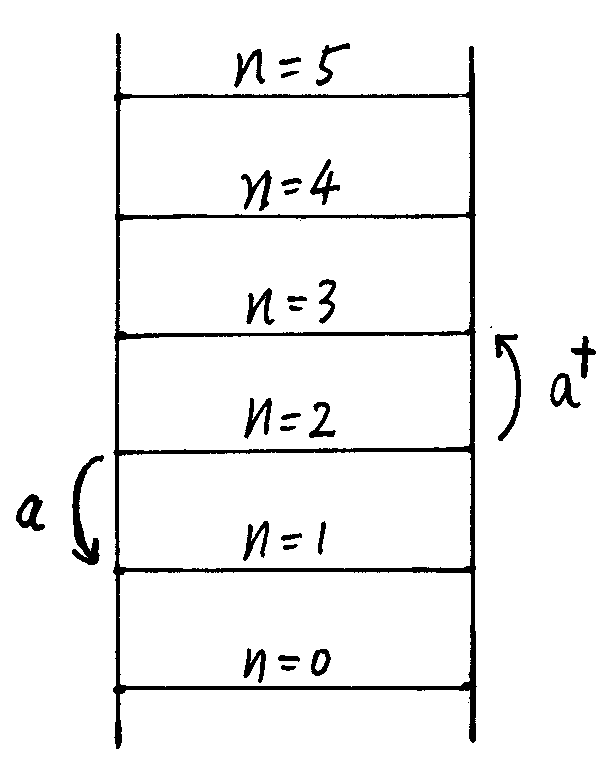
\includegraphics[width=5cm]{LinearOscillator/ladder.png}
\caption{能量的阶梯。}
\label{default}
\end{center}
\end{figure}

$E_n = \left( n + \frac{1}{2}  \right) \hbar \omega$构成了一个能量的台阶,每上一个台阶,就是多了个$\hbar \omega$能量的激发,相应地会多一份$\hbar \omega$的能量,当然第0级,或基态本身会有个非零的零点能$\frac{\hbar \omega}{2}$,因此这个能量的阶梯就是:

\begin{equation*}
\frac{\hbar \omega}{2}, \frac{3 \hbar \omega}{2}, \frac{5 \hbar \omega}{2}, \frac{7 \hbar \omega}{2}, ......
\end{equation*}

\subsection*{练习}

\begin{enumerate}
\item 

分辨一个$10^{-15}$米的结构,我们至少需要使用什么能量的光子?

\item

对线性谐振子的哈密顿量,利用海森堡运动方程分别计算$\dot X$,$\dot P$,$\dot a$和$\dot a^\dagger$

\end{enumerate}



